%% ENGR114_lab_assignment.tplx %%
%
% Built off of the article.tplx template %


% Default to the notebook output style

    


% Inherit from the specified cell style.




    
    \documentclass[11pt]{article}

    
    
    %% installed packages_rev2.tplx %%

\usepackage{fancyhdr}
\usepackage{lastpage}
\usepackage{framed,color}
\definecolor{shadecolor}{rgb}{.8,.8,.8}
\usepackage{titlesec}
% no indent on any paragraphs, vertical spacing between paragraphs is set to 1em
\usepackage[]{parskip}  % add [skip=1em] if the compiler will allow.

% for MATLAB syntax highlighting
\usepackage{listings}             % Include the listings-package
\definecolor{mygray}{rgb}{0.8,0.8,0.8} % color values Red, Green, Blue
\definecolor{mygreen}{RGB}{28,172,0}
\definecolor{mylilas}{RGB}{170,55,241}
    
    \usepackage[T1]{fontenc}
    % Nicer default font (+ math font) than Computer Modern for most use cases
    \usepackage{mathpazo}

    % Basic figure setup, for now with no caption control since it's done
    % automatically by Pandoc (which extracts ![](path) syntax from Markdown).
    \usepackage{graphicx}
    % We will generate all images so they have a width \maxwidth. This means
    % that they will get their normal width if they fit onto the page, but
    % are scaled down if they would overflow the margins.
    \makeatletter
    \def\maxwidth{\ifdim\Gin@nat@width>\linewidth\linewidth
    \else\Gin@nat@width\fi}
    \makeatother
    \let\Oldincludegraphics\includegraphics
    % Set max figure width to be 80% of text width, for now hardcoded.
    \renewcommand{\includegraphics}[1]{\Oldincludegraphics[width=.8\maxwidth]{#1}}
    % Ensure that by default, figures have no caption (until we provide a
    % proper Figure object with a Caption API and a way to capture that
    % in the conversion process - todo).
    \usepackage{caption}
    \DeclareCaptionLabelFormat{nolabel}{}
    \captionsetup{labelformat=nolabel}

    \usepackage{adjustbox} % Used to constrain images to a maximum size 
    \usepackage{xcolor} % Allow colors to be defined
    \usepackage{enumerate} % Needed for markdown enumerations to work
    \usepackage{geometry} % Used to adjust the document margins
    \usepackage{amsmath} % Equations
    \usepackage{amssymb} % Equations
    \usepackage{textcomp} % defines textquotesingle
    % Hack from http://tex.stackexchange.com/a/47451/13684:
    \AtBeginDocument{%
        \def\PYZsq{\textquotesingle}% Upright quotes in Pygmentized code
    }
    \usepackage{upquote} % Upright quotes for verbatim code
    \usepackage{eurosym} % defines \euro
    \usepackage[mathletters]{ucs} % Extended unicode (utf-8) support
    \usepackage[utf8x]{inputenc} % Allow utf-8 characters in the tex document
    \usepackage{fancyvrb} % verbatim replacement that allows latex
    \usepackage{grffile} % extends the file name processing of package graphics 
                         % to support a larger range 
    % The hyperref package gives us a pdf with properly built
    % internal navigation ('pdf bookmarks' for the table of contents,
    % internal cross-reference links, web links for URLs, etc.)
    \usepackage{hyperref}
    \usepackage{longtable} % longtable support required by pandoc >1.10
    \usepackage{booktabs}  % table support for pandoc > 1.12.2
    \usepackage[inline]{enumitem} % IRkernel/repr support (it uses the enumerate* environment)
    \usepackage[normalem]{ulem} % ulem is needed to support strikethroughs (\sout)
                                % normalem makes italics be italics, not underlines
    


    
    %% lab_title.tplx %% 
 
\newcommand{\labtitle}{Project Requirements} 
    %% header_and_footer.tplx %%

% Header and Footer
\lhead{\textbf{\labtitle}}
\rhead{ENGR114 Engineering Programming}
\lfoot{Portland Community College, \the\year}
\cfoot{}
\rfoot{\thepage~of~\pageref{LastPage}}  % must compile twice for LastPage

%lines below header and above footer
\renewcommand{\headrulewidth}{0.4pt}
\renewcommand{\footrulewidth}{0.4pt}

% Tabs
\newcommand{\itab}[1]{\hspace{0em}\rlap{#1}}
\newcommand{\tab}[1]{\hspace{.4\textwidth}\rlap{#1}}
\newcommand{\tabA}[1]{\hspace{.2\textwidth}\rlap{#1}}
    %% title_sec_formatting.tplx %%

\titleformat{\section}[block]{\LARGE\bfseries\filcenter}{}{1em}{}

\titleformat{\subsection}[hang]{\Large\bfseries}{}{1em}{}
\titlespacing{\subsection}{-1.4em}{1.5em}{1em}

\titleformat{\subsubsection}[hang]{\large\bfseries}{}{1em}{}
\titlespacing{\subsubsection}{-1.1em}{1.5em}{0.8em}
    
        \title{Problem Solving 101 with Python}
        \author{Peter D. Kazarinoff, PhD}
        \date{}
    
    
    
    % Colors for the hyperref package
    \definecolor{urlcolor}{rgb}{0,.145,.698}
    \definecolor{linkcolor}{rgb}{.71,0.21,0.01}
    \definecolor{citecolor}{rgb}{.12,.54,.11}

    % ANSI colors
    \definecolor{ansi-black}{HTML}{3E424D}
    \definecolor{ansi-black-intense}{HTML}{282C36}
    \definecolor{ansi-red}{HTML}{E75C58}
    \definecolor{ansi-red-intense}{HTML}{B22B31}
    \definecolor{ansi-green}{HTML}{00A250}
    \definecolor{ansi-green-intense}{HTML}{007427}
    \definecolor{ansi-yellow}{HTML}{DDB62B}
    \definecolor{ansi-yellow-intense}{HTML}{B27D12}
    \definecolor{ansi-blue}{HTML}{208FFB}
    \definecolor{ansi-blue-intense}{HTML}{0065CA}
    \definecolor{ansi-magenta}{HTML}{D160C4}
    \definecolor{ansi-magenta-intense}{HTML}{A03196}
    \definecolor{ansi-cyan}{HTML}{60C6C8}
    \definecolor{ansi-cyan-intense}{HTML}{258F8F}
    \definecolor{ansi-white}{HTML}{C5C1B4}
    \definecolor{ansi-white-intense}{HTML}{A1A6B2}

    % commands and environments needed by pandoc snippets
    % extracted from the output of `pandoc -s`
    \providecommand{\tightlist}{%
      \setlength{\itemsep}{0pt}\setlength{\parskip}{0pt}}
    \DefineVerbatimEnvironment{Highlighting}{Verbatim}{commandchars=\\\{\}}
    % Add ',fontsize=\small' for more characters per line
    \newenvironment{Shaded}{}{}
    \newcommand{\KeywordTok}[1]{\textcolor[rgb]{0.00,0.44,0.13}{\textbf{{#1}}}}
    \newcommand{\DataTypeTok}[1]{\textcolor[rgb]{0.56,0.13,0.00}{{#1}}}
    \newcommand{\DecValTok}[1]{\textcolor[rgb]{0.25,0.63,0.44}{{#1}}}
    \newcommand{\BaseNTok}[1]{\textcolor[rgb]{0.25,0.63,0.44}{{#1}}}
    \newcommand{\FloatTok}[1]{\textcolor[rgb]{0.25,0.63,0.44}{{#1}}}
    \newcommand{\CharTok}[1]{\textcolor[rgb]{0.25,0.44,0.63}{{#1}}}
    \newcommand{\StringTok}[1]{\textcolor[rgb]{0.25,0.44,0.63}{{#1}}}
    \newcommand{\CommentTok}[1]{\textcolor[rgb]{0.38,0.63,0.69}{\textit{{#1}}}}
    \newcommand{\OtherTok}[1]{\textcolor[rgb]{0.00,0.44,0.13}{{#1}}}
    \newcommand{\AlertTok}[1]{\textcolor[rgb]{1.00,0.00,0.00}{\textbf{{#1}}}}
    \newcommand{\FunctionTok}[1]{\textcolor[rgb]{0.02,0.16,0.49}{{#1}}}
    \newcommand{\RegionMarkerTok}[1]{{#1}}
    \newcommand{\ErrorTok}[1]{\textcolor[rgb]{1.00,0.00,0.00}{\textbf{{#1}}}}
    \newcommand{\NormalTok}[1]{{#1}}
    
    % Additional commands for more recent versions of Pandoc
    \newcommand{\ConstantTok}[1]{\textcolor[rgb]{0.53,0.00,0.00}{{#1}}}
    \newcommand{\SpecialCharTok}[1]{\textcolor[rgb]{0.25,0.44,0.63}{{#1}}}
    \newcommand{\VerbatimStringTok}[1]{\textcolor[rgb]{0.25,0.44,0.63}{{#1}}}
    \newcommand{\SpecialStringTok}[1]{\textcolor[rgb]{0.73,0.40,0.53}{{#1}}}
    \newcommand{\ImportTok}[1]{{#1}}
    \newcommand{\DocumentationTok}[1]{\textcolor[rgb]{0.73,0.13,0.13}{\textit{{#1}}}}
    \newcommand{\AnnotationTok}[1]{\textcolor[rgb]{0.38,0.63,0.69}{\textbf{\textit{{#1}}}}}
    \newcommand{\CommentVarTok}[1]{\textcolor[rgb]{0.38,0.63,0.69}{\textbf{\textit{{#1}}}}}
    \newcommand{\VariableTok}[1]{\textcolor[rgb]{0.10,0.09,0.49}{{#1}}}
    \newcommand{\ControlFlowTok}[1]{\textcolor[rgb]{0.00,0.44,0.13}{\textbf{{#1}}}}
    \newcommand{\OperatorTok}[1]{\textcolor[rgb]{0.40,0.40,0.40}{{#1}}}
    \newcommand{\BuiltInTok}[1]{{#1}}
    \newcommand{\ExtensionTok}[1]{{#1}}
    \newcommand{\PreprocessorTok}[1]{\textcolor[rgb]{0.74,0.48,0.00}{{#1}}}
    \newcommand{\AttributeTok}[1]{\textcolor[rgb]{0.49,0.56,0.16}{{#1}}}
    \newcommand{\InformationTok}[1]{\textcolor[rgb]{0.38,0.63,0.69}{\textbf{\textit{{#1}}}}}
    \newcommand{\WarningTok}[1]{\textcolor[rgb]{0.38,0.63,0.69}{\textbf{\textit{{#1}}}}}
    
    
    % Define a nice break command that doesn't care if a line doesn't already
    % exist.
    \def\br{\hspace*{\fill} \\* }
    % Math Jax compatability definitions
    \def\gt{>}
    \def\lt{<}
    % Document parameters
    
        \title{Problem Solving 101 with Python}
        \author{Peter D. Kazarinoff, PhD}
        \date{}
    
    
    
    

    % Pygments definitions
    
\makeatletter
\def\PY@reset{\let\PY@it=\relax \let\PY@bf=\relax%
    \let\PY@ul=\relax \let\PY@tc=\relax%
    \let\PY@bc=\relax \let\PY@ff=\relax}
\def\PY@tok#1{\csname PY@tok@#1\endcsname}
\def\PY@toks#1+{\ifx\relax#1\empty\else%
    \PY@tok{#1}\expandafter\PY@toks\fi}
\def\PY@do#1{\PY@bc{\PY@tc{\PY@ul{%
    \PY@it{\PY@bf{\PY@ff{#1}}}}}}}
\def\PY#1#2{\PY@reset\PY@toks#1+\relax+\PY@do{#2}}

\expandafter\def\csname PY@tok@w\endcsname{\def\PY@tc##1{\textcolor[rgb]{0.73,0.73,0.73}{##1}}}
\expandafter\def\csname PY@tok@c\endcsname{\let\PY@it=\textit\def\PY@tc##1{\textcolor[rgb]{0.25,0.50,0.50}{##1}}}
\expandafter\def\csname PY@tok@cp\endcsname{\def\PY@tc##1{\textcolor[rgb]{0.74,0.48,0.00}{##1}}}
\expandafter\def\csname PY@tok@k\endcsname{\let\PY@bf=\textbf\def\PY@tc##1{\textcolor[rgb]{0.00,0.50,0.00}{##1}}}
\expandafter\def\csname PY@tok@kp\endcsname{\def\PY@tc##1{\textcolor[rgb]{0.00,0.50,0.00}{##1}}}
\expandafter\def\csname PY@tok@kt\endcsname{\def\PY@tc##1{\textcolor[rgb]{0.69,0.00,0.25}{##1}}}
\expandafter\def\csname PY@tok@o\endcsname{\def\PY@tc##1{\textcolor[rgb]{0.40,0.40,0.40}{##1}}}
\expandafter\def\csname PY@tok@ow\endcsname{\let\PY@bf=\textbf\def\PY@tc##1{\textcolor[rgb]{0.67,0.13,1.00}{##1}}}
\expandafter\def\csname PY@tok@nb\endcsname{\def\PY@tc##1{\textcolor[rgb]{0.00,0.50,0.00}{##1}}}
\expandafter\def\csname PY@tok@nf\endcsname{\def\PY@tc##1{\textcolor[rgb]{0.00,0.00,1.00}{##1}}}
\expandafter\def\csname PY@tok@nc\endcsname{\let\PY@bf=\textbf\def\PY@tc##1{\textcolor[rgb]{0.00,0.00,1.00}{##1}}}
\expandafter\def\csname PY@tok@nn\endcsname{\let\PY@bf=\textbf\def\PY@tc##1{\textcolor[rgb]{0.00,0.00,1.00}{##1}}}
\expandafter\def\csname PY@tok@ne\endcsname{\let\PY@bf=\textbf\def\PY@tc##1{\textcolor[rgb]{0.82,0.25,0.23}{##1}}}
\expandafter\def\csname PY@tok@nv\endcsname{\def\PY@tc##1{\textcolor[rgb]{0.10,0.09,0.49}{##1}}}
\expandafter\def\csname PY@tok@no\endcsname{\def\PY@tc##1{\textcolor[rgb]{0.53,0.00,0.00}{##1}}}
\expandafter\def\csname PY@tok@nl\endcsname{\def\PY@tc##1{\textcolor[rgb]{0.63,0.63,0.00}{##1}}}
\expandafter\def\csname PY@tok@ni\endcsname{\let\PY@bf=\textbf\def\PY@tc##1{\textcolor[rgb]{0.60,0.60,0.60}{##1}}}
\expandafter\def\csname PY@tok@na\endcsname{\def\PY@tc##1{\textcolor[rgb]{0.49,0.56,0.16}{##1}}}
\expandafter\def\csname PY@tok@nt\endcsname{\let\PY@bf=\textbf\def\PY@tc##1{\textcolor[rgb]{0.00,0.50,0.00}{##1}}}
\expandafter\def\csname PY@tok@nd\endcsname{\def\PY@tc##1{\textcolor[rgb]{0.67,0.13,1.00}{##1}}}
\expandafter\def\csname PY@tok@s\endcsname{\def\PY@tc##1{\textcolor[rgb]{0.73,0.13,0.13}{##1}}}
\expandafter\def\csname PY@tok@sd\endcsname{\let\PY@it=\textit\def\PY@tc##1{\textcolor[rgb]{0.73,0.13,0.13}{##1}}}
\expandafter\def\csname PY@tok@si\endcsname{\let\PY@bf=\textbf\def\PY@tc##1{\textcolor[rgb]{0.73,0.40,0.53}{##1}}}
\expandafter\def\csname PY@tok@se\endcsname{\let\PY@bf=\textbf\def\PY@tc##1{\textcolor[rgb]{0.73,0.40,0.13}{##1}}}
\expandafter\def\csname PY@tok@sr\endcsname{\def\PY@tc##1{\textcolor[rgb]{0.73,0.40,0.53}{##1}}}
\expandafter\def\csname PY@tok@ss\endcsname{\def\PY@tc##1{\textcolor[rgb]{0.10,0.09,0.49}{##1}}}
\expandafter\def\csname PY@tok@sx\endcsname{\def\PY@tc##1{\textcolor[rgb]{0.00,0.50,0.00}{##1}}}
\expandafter\def\csname PY@tok@m\endcsname{\def\PY@tc##1{\textcolor[rgb]{0.40,0.40,0.40}{##1}}}
\expandafter\def\csname PY@tok@gh\endcsname{\let\PY@bf=\textbf\def\PY@tc##1{\textcolor[rgb]{0.00,0.00,0.50}{##1}}}
\expandafter\def\csname PY@tok@gu\endcsname{\let\PY@bf=\textbf\def\PY@tc##1{\textcolor[rgb]{0.50,0.00,0.50}{##1}}}
\expandafter\def\csname PY@tok@gd\endcsname{\def\PY@tc##1{\textcolor[rgb]{0.63,0.00,0.00}{##1}}}
\expandafter\def\csname PY@tok@gi\endcsname{\def\PY@tc##1{\textcolor[rgb]{0.00,0.63,0.00}{##1}}}
\expandafter\def\csname PY@tok@gr\endcsname{\def\PY@tc##1{\textcolor[rgb]{1.00,0.00,0.00}{##1}}}
\expandafter\def\csname PY@tok@ge\endcsname{\let\PY@it=\textit}
\expandafter\def\csname PY@tok@gs\endcsname{\let\PY@bf=\textbf}
\expandafter\def\csname PY@tok@gp\endcsname{\let\PY@bf=\textbf\def\PY@tc##1{\textcolor[rgb]{0.00,0.00,0.50}{##1}}}
\expandafter\def\csname PY@tok@go\endcsname{\def\PY@tc##1{\textcolor[rgb]{0.53,0.53,0.53}{##1}}}
\expandafter\def\csname PY@tok@gt\endcsname{\def\PY@tc##1{\textcolor[rgb]{0.00,0.27,0.87}{##1}}}
\expandafter\def\csname PY@tok@err\endcsname{\def\PY@bc##1{\setlength{\fboxsep}{0pt}\fcolorbox[rgb]{1.00,0.00,0.00}{1,1,1}{\strut ##1}}}
\expandafter\def\csname PY@tok@kc\endcsname{\let\PY@bf=\textbf\def\PY@tc##1{\textcolor[rgb]{0.00,0.50,0.00}{##1}}}
\expandafter\def\csname PY@tok@kd\endcsname{\let\PY@bf=\textbf\def\PY@tc##1{\textcolor[rgb]{0.00,0.50,0.00}{##1}}}
\expandafter\def\csname PY@tok@kn\endcsname{\let\PY@bf=\textbf\def\PY@tc##1{\textcolor[rgb]{0.00,0.50,0.00}{##1}}}
\expandafter\def\csname PY@tok@kr\endcsname{\let\PY@bf=\textbf\def\PY@tc##1{\textcolor[rgb]{0.00,0.50,0.00}{##1}}}
\expandafter\def\csname PY@tok@bp\endcsname{\def\PY@tc##1{\textcolor[rgb]{0.00,0.50,0.00}{##1}}}
\expandafter\def\csname PY@tok@fm\endcsname{\def\PY@tc##1{\textcolor[rgb]{0.00,0.00,1.00}{##1}}}
\expandafter\def\csname PY@tok@vc\endcsname{\def\PY@tc##1{\textcolor[rgb]{0.10,0.09,0.49}{##1}}}
\expandafter\def\csname PY@tok@vg\endcsname{\def\PY@tc##1{\textcolor[rgb]{0.10,0.09,0.49}{##1}}}
\expandafter\def\csname PY@tok@vi\endcsname{\def\PY@tc##1{\textcolor[rgb]{0.10,0.09,0.49}{##1}}}
\expandafter\def\csname PY@tok@vm\endcsname{\def\PY@tc##1{\textcolor[rgb]{0.10,0.09,0.49}{##1}}}
\expandafter\def\csname PY@tok@sa\endcsname{\def\PY@tc##1{\textcolor[rgb]{0.73,0.13,0.13}{##1}}}
\expandafter\def\csname PY@tok@sb\endcsname{\def\PY@tc##1{\textcolor[rgb]{0.73,0.13,0.13}{##1}}}
\expandafter\def\csname PY@tok@sc\endcsname{\def\PY@tc##1{\textcolor[rgb]{0.73,0.13,0.13}{##1}}}
\expandafter\def\csname PY@tok@dl\endcsname{\def\PY@tc##1{\textcolor[rgb]{0.73,0.13,0.13}{##1}}}
\expandafter\def\csname PY@tok@s2\endcsname{\def\PY@tc##1{\textcolor[rgb]{0.73,0.13,0.13}{##1}}}
\expandafter\def\csname PY@tok@sh\endcsname{\def\PY@tc##1{\textcolor[rgb]{0.73,0.13,0.13}{##1}}}
\expandafter\def\csname PY@tok@s1\endcsname{\def\PY@tc##1{\textcolor[rgb]{0.73,0.13,0.13}{##1}}}
\expandafter\def\csname PY@tok@mb\endcsname{\def\PY@tc##1{\textcolor[rgb]{0.40,0.40,0.40}{##1}}}
\expandafter\def\csname PY@tok@mf\endcsname{\def\PY@tc##1{\textcolor[rgb]{0.40,0.40,0.40}{##1}}}
\expandafter\def\csname PY@tok@mh\endcsname{\def\PY@tc##1{\textcolor[rgb]{0.40,0.40,0.40}{##1}}}
\expandafter\def\csname PY@tok@mi\endcsname{\def\PY@tc##1{\textcolor[rgb]{0.40,0.40,0.40}{##1}}}
\expandafter\def\csname PY@tok@il\endcsname{\def\PY@tc##1{\textcolor[rgb]{0.40,0.40,0.40}{##1}}}
\expandafter\def\csname PY@tok@mo\endcsname{\def\PY@tc##1{\textcolor[rgb]{0.40,0.40,0.40}{##1}}}
\expandafter\def\csname PY@tok@ch\endcsname{\let\PY@it=\textit\def\PY@tc##1{\textcolor[rgb]{0.25,0.50,0.50}{##1}}}
\expandafter\def\csname PY@tok@cm\endcsname{\let\PY@it=\textit\def\PY@tc##1{\textcolor[rgb]{0.25,0.50,0.50}{##1}}}
\expandafter\def\csname PY@tok@cpf\endcsname{\let\PY@it=\textit\def\PY@tc##1{\textcolor[rgb]{0.25,0.50,0.50}{##1}}}
\expandafter\def\csname PY@tok@c1\endcsname{\let\PY@it=\textit\def\PY@tc##1{\textcolor[rgb]{0.25,0.50,0.50}{##1}}}
\expandafter\def\csname PY@tok@cs\endcsname{\let\PY@it=\textit\def\PY@tc##1{\textcolor[rgb]{0.25,0.50,0.50}{##1}}}

\def\PYZbs{\char`\\}
\def\PYZus{\char`\_}
\def\PYZob{\char`\{}
\def\PYZcb{\char`\}}
\def\PYZca{\char`\^}
\def\PYZam{\char`\&}
\def\PYZlt{\char`\<}
\def\PYZgt{\char`\>}
\def\PYZsh{\char`\#}
\def\PYZpc{\char`\%}
\def\PYZdl{\char`\$}
\def\PYZhy{\char`\-}
\def\PYZsq{\char`\'}
\def\PYZdq{\char`\"}
\def\PYZti{\char`\~}
% for compatibility with earlier versions
\def\PYZat{@}
\def\PYZlb{[}
\def\PYZrb{]}
\makeatother


    % Exact colors from NB
    \definecolor{incolor}{rgb}{0.0, 0.0, 0.5}
    \definecolor{outcolor}{rgb}{0.545, 0.0, 0.0}




    
    % Prevent overflowing lines due to hard-to-break entities
    \sloppy 
    % Setup hyperref package
    \hypersetup{
      breaklinks=true,  % so long urls are correctly broken across lines
      colorlinks=true,
      urlcolor=urlcolor,
      linkcolor=linkcolor,
      citecolor=citecolor,
      }
    % Slightly bigger margins than the latex defaults
    
    %% margins.tplx %%

% margins
\textwidth=7in
\textheight=9.0in
\topmargin=-0.5in
\headheight=15pt
\headsep=.5in
\hoffset = -0.5in

\pagestyle{fancy}

    

    \begin{document}
    
    
    

    
    

    
    \hypertarget{group-project-requirements}{%
\section{Group Project Requirements}\label{group-project-requirements}}

    \hypertarget{background}{%
\subsection{Background}\label{background}}

    The Engineering Lab in AM103 has a set of computers with MATLAB
installed and is a great place for students to go when working on
homework, projects or studying. In the Engineering Lab there is also a
hydroponic garden / fish tank installation. The fish produce nutrients
for the plants and the plants clean the water for the fish. Water from
the fish tank is pumped up to the plants. The plants and soil filter the
water before it flows back down; clean and oxygenated into the tank. For
this cycle to continue working, the fish tank needs a pump to move the
water and the plants need a grow light for photosynthesis. Both of these
are currently plugged into the wall and need to be turned on manually by
a lab technician. A great system for fish and plants, but what a pain
for the lab technician. And who is going to turn on the pump and grow
light during weekends and breaks?

    \begin{figure}[h!]
\centering
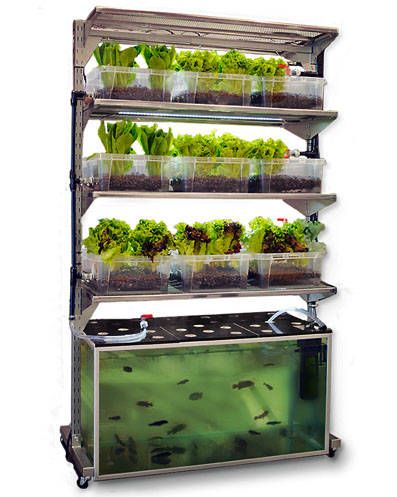
\includegraphics{images/image1.jpg}
\caption{Hydroponic Garden and Fishtank}
\end{figure}

    Wouldn't it be better if the system was smart and automated? Wouldn't it
be better if the the pump only turned on when it was needed and the
light automatically turned on during daylight hours? One way to
accomplish this is with programming!

    In order to make an automated system that can be monitored remotely, a
couple of pieces of hardware is needed. One type of hardware needed are
sensors. Sensors that can measure the temperature, pH and water depth in
the fish tank could help determine when the pump needs to be turned on.
A sensor that can measure light level could help determine when to turn
on the grow light. The light and the pump need some additional hardware
too. Both of these need to be connected to relays so that a small signal
current can control the high current light and pump. These sensors and
relays need to be connected to microcontrollers so that they con be
integrated with a computer.

    \hypertarget{arduio-iot-micropython-project}{%
\subsection{Arduio IoT / MicroPython
Project}\label{arduio-iot-micropython-project}}

    For this group project, your group will use Python to interact an
Arduino (or use MicroPython on a different microcontroller) to
dynamically collect sensor data or control a relay and post the data or
relay state on ThingSpeak (an IoT cloud server). Each group will be
tasked with reading or controlling one of the following: Light Sensor,
pH Sensor, Fish Feeder motor, Light Relay or Pump Relay.

    In order for your group to accomplish this task, your hardware will need
to do a couple of things:

    \begin{enumerate}
\def\labelenumi{\arabic{enumi}.}
\tightlist
\item
  The sensor, relay or motor needs to be mounted on or near the fish
  tank in order to record data or flip a switch
\item
  An Arduino or a microcontroller with MicroPython connected to the
  sensor or relay either directly or through some other hardware on a
  breadboard will record the raw voltage value coming from the sensor
  and sent it to a laptop
\item
  A laptop with Python installed, connected to the Arduino or
  microcontroller with a USB cable, will read in the sensor data and
  process it so that it can be sent to an IoT (Internet of Things)
  server.
\item
  A wireless network is needed for the Laptop to connect to. PCC's
  wireless network is available to all registered students.
\item
  An account on ThinkSpeak.com (an IoT cloud server) where the sensor
  data or relay state will be stored
\end{enumerate}

    To complete this group project, your group will need to complete a
couple of tasks

\begin{enumerate}
\def\labelenumi{\arabic{enumi}.}
\tightlist
\item
  Prototype and build the hardware to connect the sensor, motor or relay
  to the Arduino or microcontroller. Take pictures of the setup and
  create a bill of materials, schematic and hookup guide.
\item
  Write and modify the code run by the Arduino or microcontroller to
  read in the sensor voltage or push a signal out to the relay or motor.
  The Arduino or microcontroller must also pass the data to the laptop
  via the serial communication protocol or read commands coming from the
  computer over serial.
\item
  Write and modify the code run by Python on the laptop to read in the
  raw data over serial from the Arduino or microcontroller. Python must
  also clean up and modify the data and send it up to ThingSpeak.com
  using a web API call and PCC's wirelss network. If your group is
  working with a relay or motor, Python needs to read the relay or motor
  state stored in the cloud at ThingSpeak.com using the web API, clean
  up the incoming data on ThingSpeak.com and send a signal over serial
  to the Arduino or microcontroller.
\item
  Document how all of the above was accomplished including a problem
  statement, hardware setup, Python code, Arduino or MicroPython code,
  future work and a license (to denote how the code can be modified and
  used later by other students).
\end{enumerate}

    You will complete this project in a group. Each group member will be
primarily responsible for creating one of the following parts:

\hypertarget{python-coder---python_code.py}{%
\paragraph{Python Coder -
python\_code.py}\label{python-coder---python_code.py}}

Python code that connects to the Arduino or microcontroller using serial
communication. The Python script needs to read in sensor data over
serial or send characters over serial to the Arduino or microcontroller.
The Python script also needs to either post the data to ThingSpeak.com
using a web API call or read the desired relay or motor state from
ThinkSpeak.com using a web API call. The Python code needs be documented
and commented so that another group can recreate the project.

\hypertarget{arduino-or-micropython-coder---ardino_code.ino-or-micropython_code.py}{%
\paragraph{Arduino or MicroPython Coder - Ardino\_code.ino or
micropython\_code.py}\label{arduino-or-micropython-coder---ardino_code.ino-or-micropython_code.py}}

An Arduino sketch uploaded to the Arduino or MicroPython script uploaded
to a microcontroller that records the sensor readings, flips a relay, or
turns on a motor and sends data out over serial. The code does not need
to be complex, Python on a laptop should do the heavy lifting. The code
needs to documented and commented so that another group can recreate the
project.

\hypertarget{hardware-assembler---hardware_setup.docx}{%
\paragraph{Hardware Assembler -
hardware\_setup.docx}\label{hardware-assembler---hardware_setup.docx}}

A word doc with a table containing the bill of materials, a schematic
diagram (can use Fritzing) showing the hardware connected together, a
hookup guide, and pictures of all the hardware connected together.
Include enough detail that it is clear how the components are connected
so that another group could recreate the project.

\hypertarget{documentation-compiler---writeup.docx}{%
\paragraph{Documentation Compiler -
WriteUp.docx}\label{documentation-compiler---writeup.docx}}

A word doc that contains a problem statement, hardware setup, the Python
and Arduino (or MicroPython) code, a results plot of at least 100 sensor
readings (or 20 relay flips, motor turns) from ThingSpeak, future work,
and a license. Use the supplied template posted on D2L. This
documentation needs to have enough detail and clarity so that another
group can recreate the project.

    \hypertarget{your-group-will-have-to-decide-on-a-couple-things}{%
\subsubsection{Your group will have to decide on a couple
things:}\label{your-group-will-have-to-decide-on-a-couple-things}}

\begin{itemize}
\tightlist
\item
  Who is going to construct each part of the Proejct?
\item
  Who's laptop computer will be running Python and connected to the
  Arduino or microcontroller?
\item
  How will your group share code, images and hardware?
\item
  Who will submit the four required files to D2L?
\item
  Is your group going to use Fritzing to build a schematic? (a little
  extra credit)
\item
  Is your group going to use Github.com to post your project? (a little
  extra credit)
\end{itemize}

    During finals week at the end of the quarter, your group will give a
demonstration of your project in action. Your group will have 1 hour to
set up before starting the demonstration. Group members must be present,
ontime and contribute to recieve full credit for the demonstration.
During the demonstration be prepared to show your project connected
together and working action for a couple minutes.

\hypertarget{during-the-demonstration-be-prepared-to-answer-the-following-questions}{%
\paragraph{During the demonstration, be prepared to answer the following
questions:}\label{during-the-demonstration-be-prepared-to-answer-the-following-questions}}

\begin{itemize}
\tightlist
\item
  What is your problem statement? What was your group trying to
  accomplish?
\item
  How is your hardware connected together. What pieces of hardware talks
  to the others and how do they communicate?
\item
  What does the Arduino or MicroPython code do? (Don't go line by line,
  but give the general idea of each section)
\item
  What does the Python code do? (Don't go line by line, but give the
  general idea of each section)
\item
  What was the hardest part of this project? What do you wish you had
  known when the project started?
\item
  What future work could another student group do to build upon your
  project?
\end{itemize}

    Make sure your group's Python and MicroPython or Arduino code is
well-commented and sectioned. Ensure the variable names are descriptive
and there is enough documentation for another group of students to reuse
the code without much trouble. Each Group's submissions for the lab
should be done by one team member (only one person per group needs to
submit, but they must submit all 4 files).

\hypertarget{upload-these-files-four-files-to-the-d2l-arduino-iot-project-uploads-folder.}{%
\paragraph{Upload these files four files to the D2L Arduino IoT Project
uploads
folder.}\label{upload-these-files-four-files-to-the-d2l-arduino-iot-project-uploads-folder.}}

\begin{itemize}
\tightlist
\item
  python\_code.py
\item
  Arduino\_code.ino or micropython\_code.py
\item
  hardware\_setup.docx
\item
  WriteUp.docx
\end{itemize}


    % Add a bibliography block to the postdoc
    
    
    
    \end{document}
